%!TEX root = ../../../adrien_gomar_phd.tex

\chapter{Convergence of Fourier-based 
time methods for turbomachinery wake passing problems}
\label{cha:limitations_convergence}

\chabstract{Theoretical results about the convergence of spectral methods 
(see e.g. \citet{Canuto2006}
for a comprehensive review) predict convergence of the numerical 
solution starting from a given number of harmonics, provided 
that the approximated function satisfies some regularity 
requirements~\cite{Zygmund1959}. 
Nevertheless, this number of harmonics is configuration-dependent 
and hardly predictable. Studies on the convergence of 
Fourier-based time methods for turbomachinery simulations 
have been previously reported in the literature, but with scattered results. 
For instance, using a frequency-domain approach, 
\citet{Vilmin2006} obtain accurate solutions 
using 5~harmonics for a compressor stage and 3~harmonics for a 
centripetal turbine stage. For a transonic compressor stage with 
forced blade vibration, \citet{ekici2010} use 
up to 7~harmonics with a time-domain harmonic balance approach. Finally, for a 
subsonic compressor stage, \citet{JSicot2012} report 
that 4~harmonics is the minimal requirement to properly capture wake interactions.. 
The goal of the present chapter is twofold: to analyze the
convergence of Fourier-based time method, 
with focus on turbomachinery applications, 
and to provide a criterion for the minimal number of harmonics 
required to achieve a specified accuracy level.}


\newpage

\section{Periodic problems with an infinite Fourier spectrum}
\label{sec:rectangular_fct}
%!TEX root = ../../../adrien_gomar_phd.tex

In fluid dynamics, the simplest model 
representative of a shock wave
is the step function. It is a discontinuous function
that may be difficult to capture for Fourier-based time methods.
The periodic step function over the period $T=1/c$ is defined as
\begin{equation}
    u_l(t) = 
    \begin{cases}
        0, & \text{if } 0 \leq t < \frac{T}{2}, \\
        1, & \text{if } \frac{T}{2} \leq t < T.
    \end{cases}
    \label{eq:inject_step}
\end{equation}

The linear advection model problem defined in 
Sec.~\ref{sec:presentation_advection} is used here to assess
the capability of the harmonic balance approach to capture
discontinuous unsteadinesses.

\begin{figure}[htp]
  \centering
  \subfigure[$N=1$]{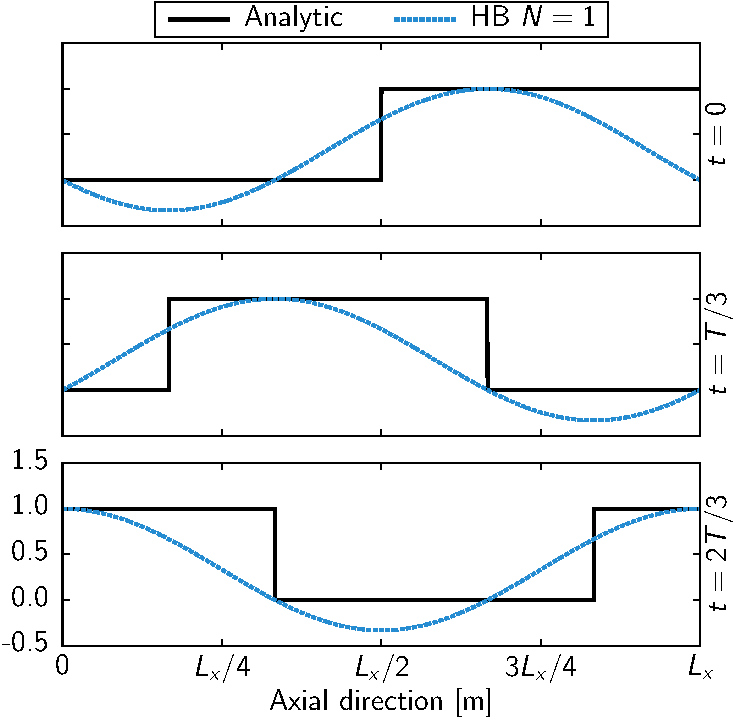
\includegraphics[width=.35\textwidth]{convection_step_N1.pdf}}
  \subfigure[$N=2$]{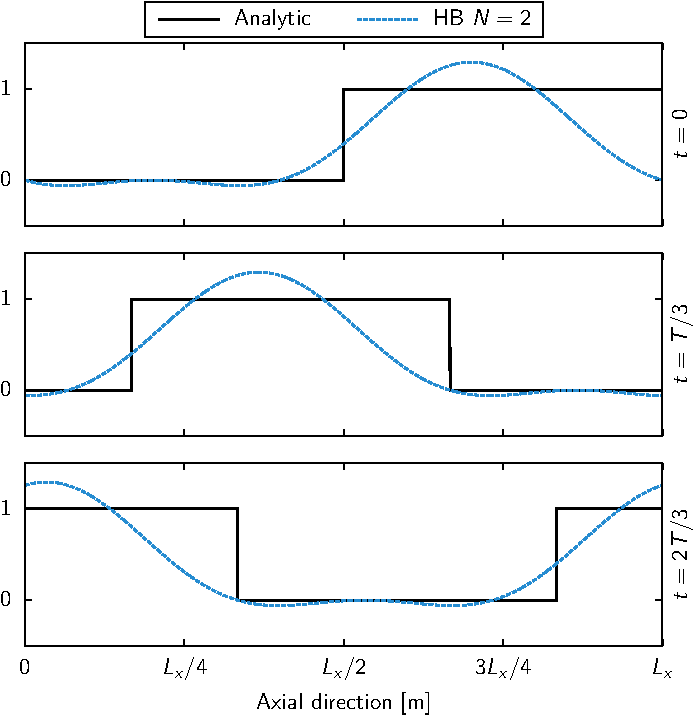
\includegraphics[width=.35\textwidth]{convection_step_N2.pdf}}
  \subfigure[$N=3$]{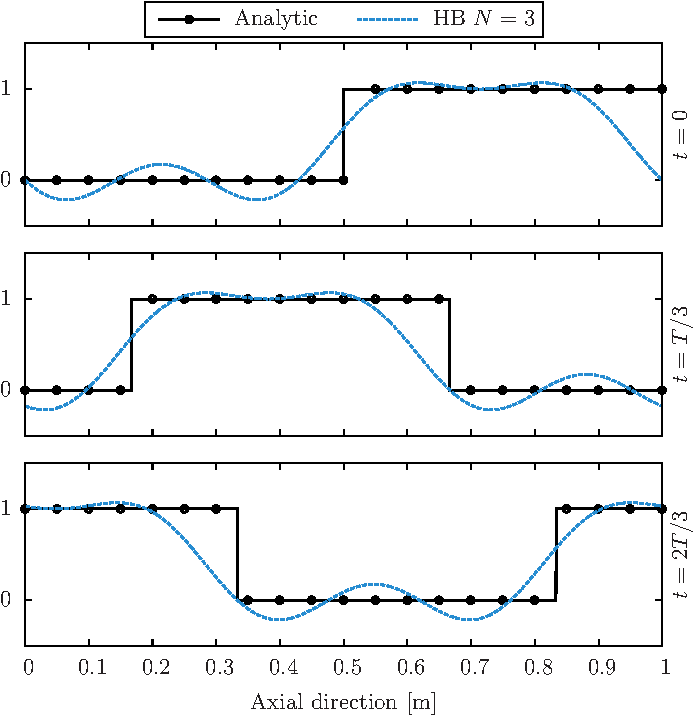
\includegraphics[width=.35\textwidth]{convection_step_N3.pdf}}
  \subfigure[$N=4$]{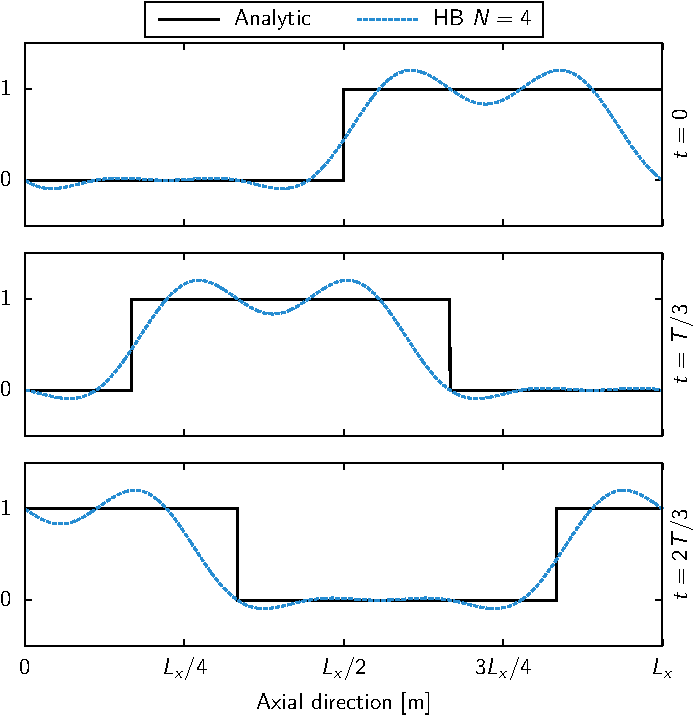
\includegraphics[width=.35\textwidth]{convection_step_N4.pdf}}
  \subfigure[$N=5$]{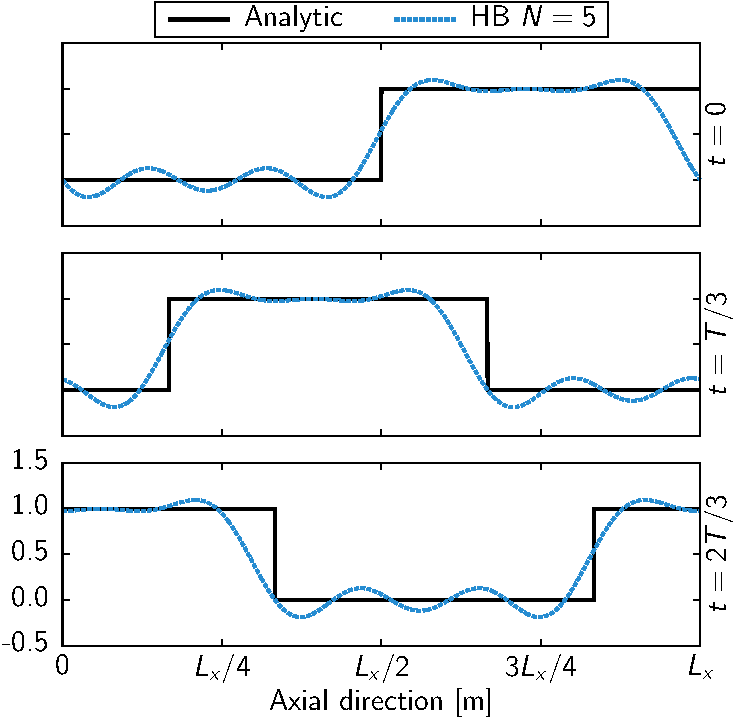
\includegraphics[width=.35\textwidth]{convection_step_N5.pdf}}
  \subfigure[$N=6$]{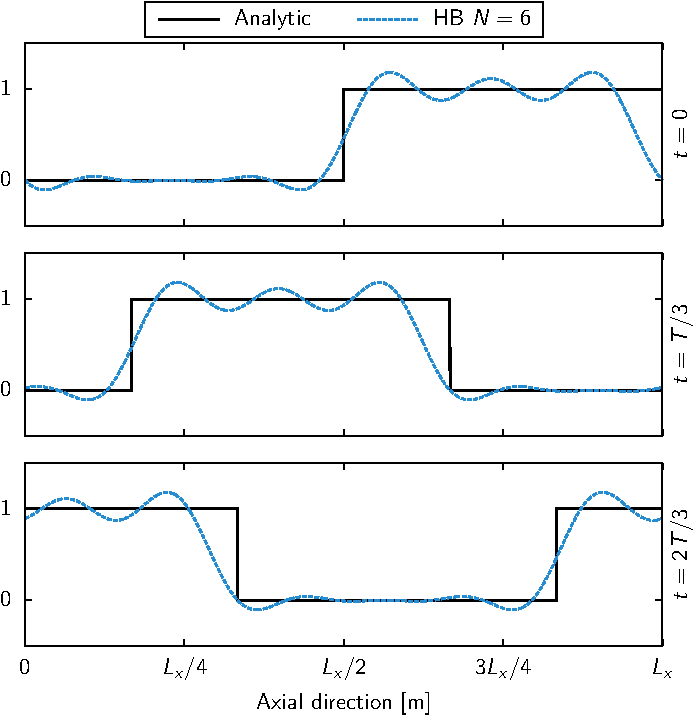
\includegraphics[width=.35\textwidth]{convection_step_N6.pdf}}
  \caption{Linear advection of a rectangular function: 
  numerical solutions at different time instances for different numbers of harmonics.}
  \label{fig:inj_step_results}
\end{figure}
Figure~\ref{fig:inj_step_results} depicts the results of HB computations
using one to six harmonics at different time instances. The convergence rate 
is slow, and for the six-harmonics HB computation the
shape of the rectangular function is still barely captured. 
The well-known \citet{Gibbs1899}
phenomenon is observed, which is a typical drawback 
of Fourier-based methods applied to discontinuous problems, 
see \emph{e.g.} \citet{Canuto2006}.

\begin{figure}[htp]
  \centering
  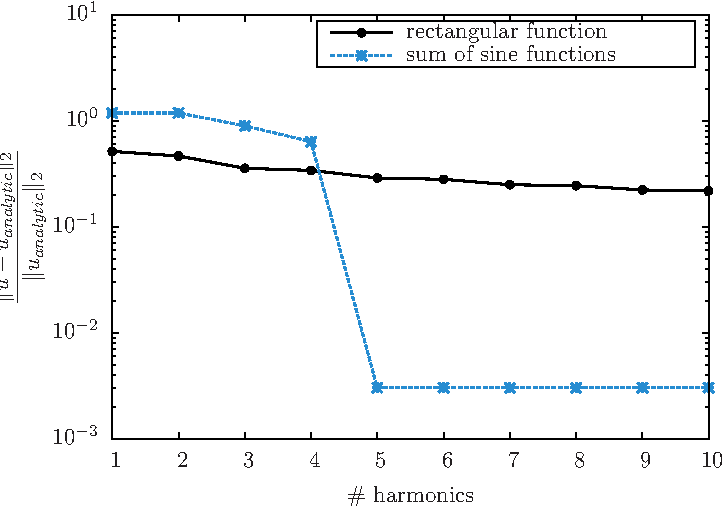
\includegraphics[width=.5\textwidth]{convection_step_error.pdf}
  \caption{Linear advection of a rectangular function: convergence of the HB method error.}
  \label{fig:conv_step}
\end{figure}
The $\mathcal{L}_2$-norm 
of the error is depicted in Figure~\ref{fig:conv_step}. 
The convergence of the sum of sine functions, 
that has been studied in Sec.~\ref{sec:sum_sine},
is added for comparison.
The convergence rate is different from the previous one: 
the error decreases slowly when more harmonics are introduced, 
but the exact solution is never reached, 
unless an infinite number of harmonics is considered.

\begin{figure}[htp]
  \centering
  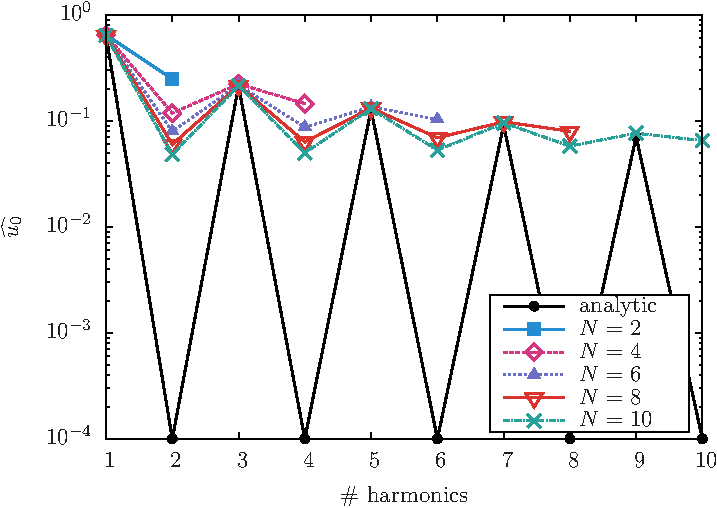
\includegraphics[width=.5\textwidth]{convection_step_dft.pdf}
  \caption{Linear advection of a rectangular function: 
  discrete Fourier transform.}
  \label{fig:dft_step}
\end{figure}
The discrete Fourier transform of the results
is computed and compared to the analytical result in Figure~\ref{fig:dft_step}.
For this case, the spectrum is not finite and cannot be captured accurately
with a finite number of samples.
Adding more harmonics improves the results but the analytical
solution is out of reach of the harmonic
balance approach. 

To summarize, Fourier-based time methods are unadapted
for unsteady signals for which the Fourier spectrum is wide.
In the next section, wake passing is modeled by an analytical
function. This allows to assess the convergence of Fourier-based time
methods for such problems.


\section{Toward turbomachinery wakes}
\label{sec:wake_fct}
%!TEX root = ../../../adrien_gomar_phd.tex

Consider for simplicity a turbomachinery stage composed of two rotors,
as for instance a CROR configuration.
A wake is shed behind the upstream rotor. 
It is stationary in the frame of reference attached to the upstream rotor.
\begin{figure}[htp]
    \centering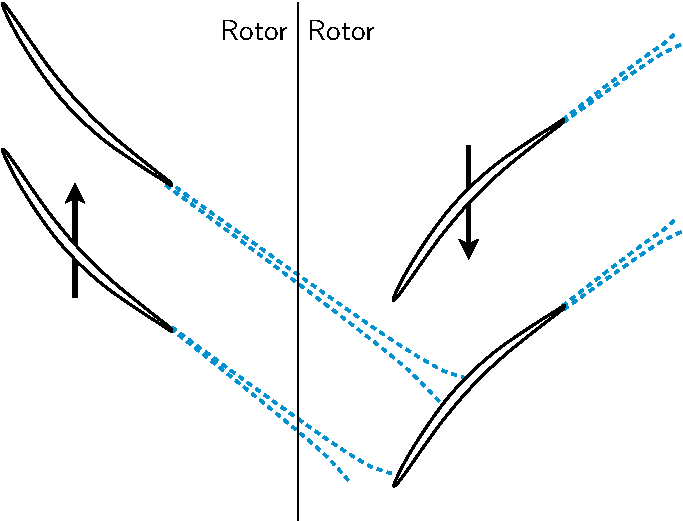
\includegraphics[width=.35\textwidth]{cror_wakes.pdf}
  \caption{Characteristic wakes in a CROR configuration.}
  \label{fig:rotor-stator}
\end{figure}
However, when it crosses the rotor/rotor interface,
the wake becomes unsteady in the frame of reference of the second wheel. 
Thus, an upstream steady spatial distortion becomes unsteady in
the downstream row.

\citet{Lakshminarayana1980} showed that the wake
behind turbomachinery blades follows a similarity law for the velocity. 
It can be empirically approximated by a Gaussian function:
\begin{equation}
    u_l (t) = u_m \left[1 - 
        \Delta u \cdot e^{
          -0.693 \left(2 \frac{\theta}{L} \right) ^ 2}\right],
    \label{eq:similarity}
\end{equation}
where $u_m$ denotes the free-stream velocity, 
$\Delta u$ the axial wake velocity deficit,
and $L$ the wake width,
defined as the full width at half maximum.
The azimuthal coordinate $\theta$ is here assimilated as $c t / L_x$.

Therefore, in the downstream frame of reference, wakes coming 
from the upstream wheel can be represented, 
to a first approximation, as the periodic 
advection of a Gaussian function from the inter-wheel interface.

To study the convergence properties of such a function,
we consider again the linear advection problem defined in Sec.~\ref{sec:linear}, 
with $u_l$ now taken equal to a Gaussian function.
The full width at half maximum $L$ of the wake is set to 10\% of the domain size, 
$u_m$ is set to $c$ and $\Delta u$ to 10\% of $u_m$.

\begin{figure}[htp]
  \centering
  \subfigure[$N=1$]{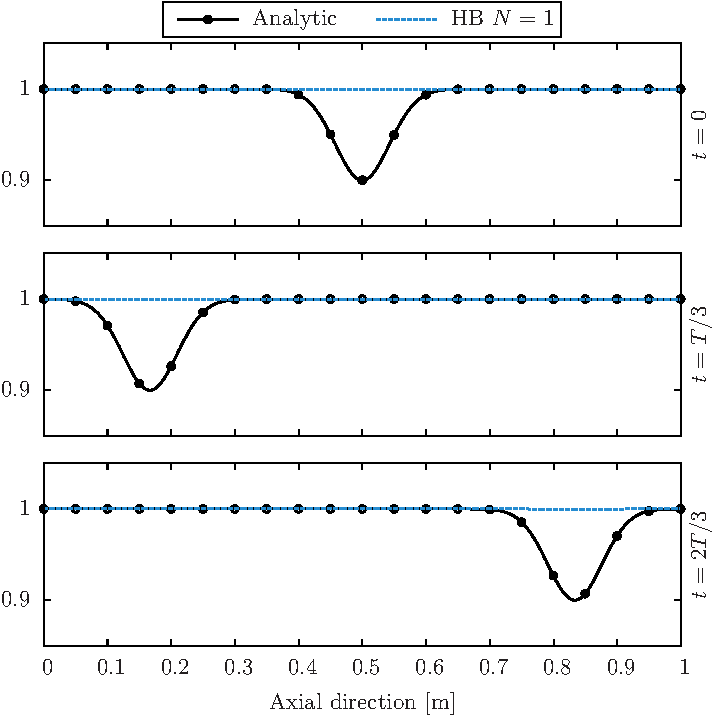
\includegraphics[width=.35\textwidth]{convection_wake_N1.pdf}}
  \subfigure[$N=2$]{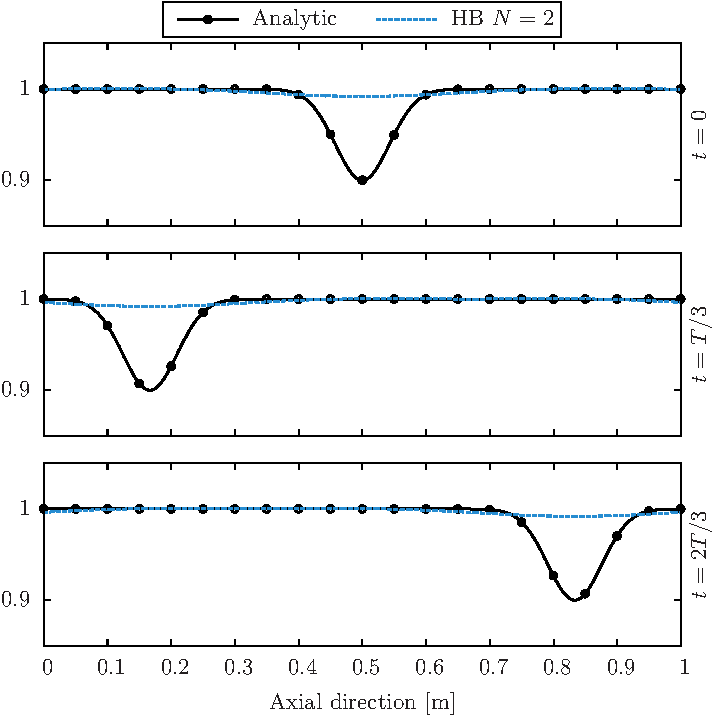
\includegraphics[width=.35\textwidth]{convection_wake_N2.pdf}}
  \subfigure[$N=3$]{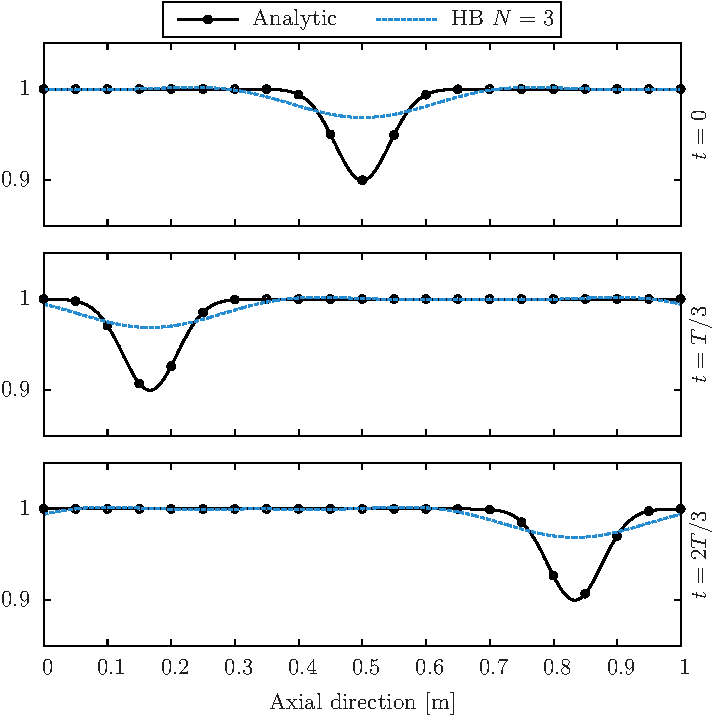
\includegraphics[width=.35\textwidth]{convection_wake_N3.pdf}}
  \subfigure[$N=4$]{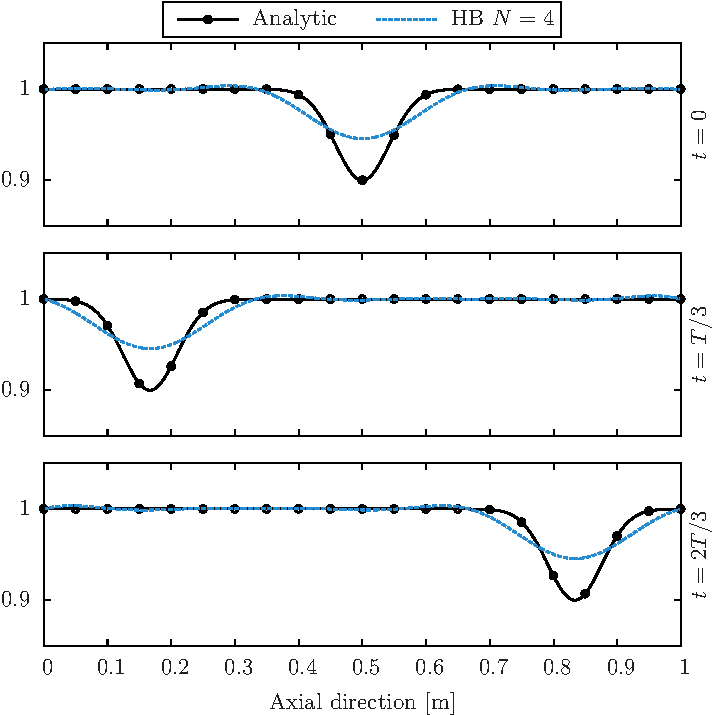
\includegraphics[width=.35\textwidth]{convection_wake_N4.pdf}}
  \subfigure[$N=5$]{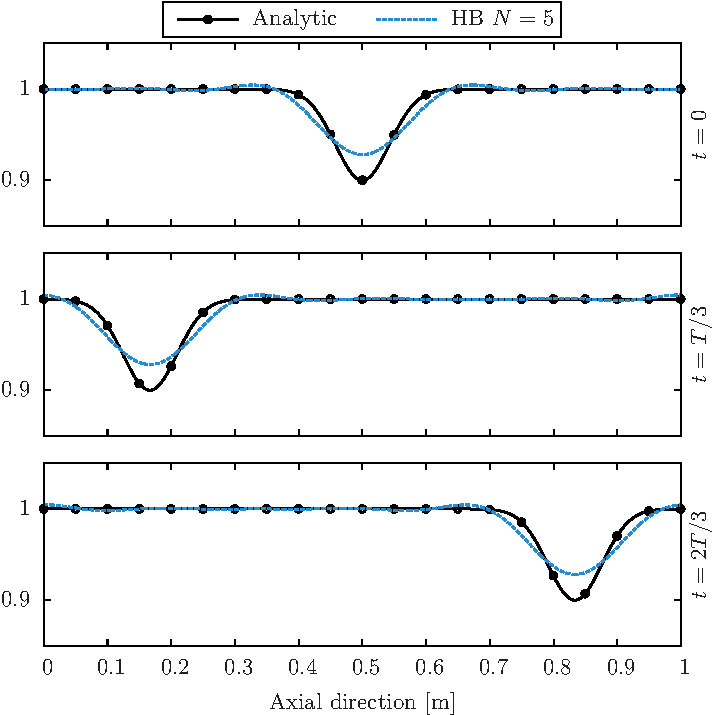
\includegraphics[width=.35\textwidth]{convection_wake_N5.pdf}}
  \subfigure[$N=6$]{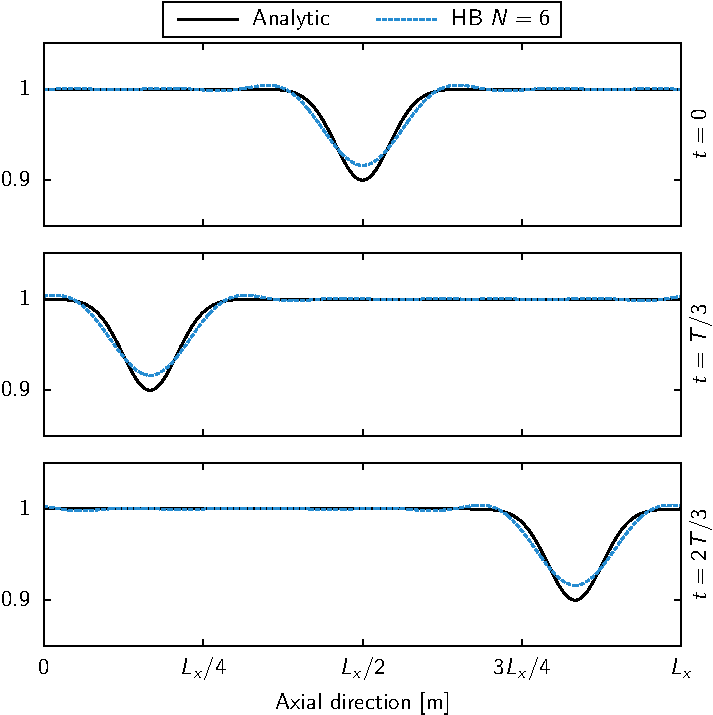
\includegraphics[width=.35\textwidth]{convection_wake_N6.pdf}}
  \caption{Linear advection of a Gaussian function representing a turbomachinery wake: 
  numerical solutions at different time instances for different numbers of harmonics.}
  \label{fig:inj_wake_results}
\end{figure}
Figure~\ref{fig:inj_wake_results} depicts the HB
computations for one to six harmonics. The numerical solution start to convergence
toward the Gaussian function starting from $N=6$ harmonics.
When the number of harmonics is
too small, the width and the depth of the wake are badly approximated
by the method, and the solution exhibits some spurious oscillations. 

\begin{figure}[htp]
  \centering
  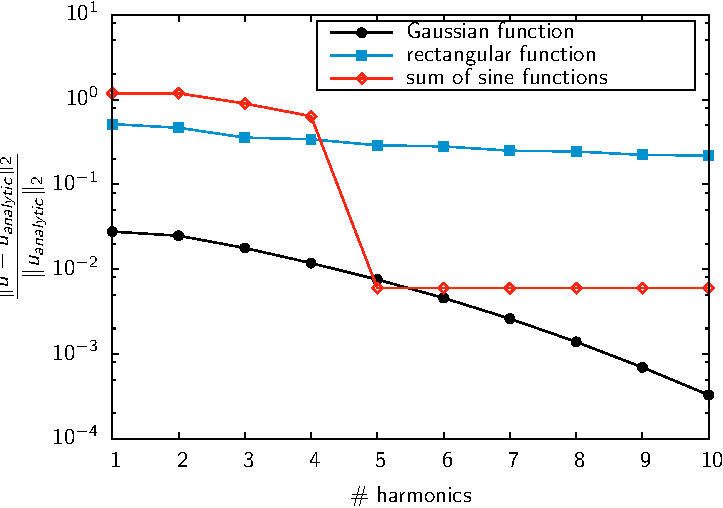
\includegraphics[width=.5\textwidth]{convection_wake_error.pdf}
  \caption{Linear advection of a Gaussian function representing a 
  turbomachinery wake: convergence of the HB method error.}
  \label{fig:conv_wake}
\end{figure}
Figure~\ref{fig:conv_wake} shows the quantitative convergence of 
the $\mathcal{L}_2$ error. The
convergence curves for the two functions studied in the previous sections
are also reported for comparison.
The error follows now a nearly exponential convergence.
\begin{figure}[htp]
  \centering
  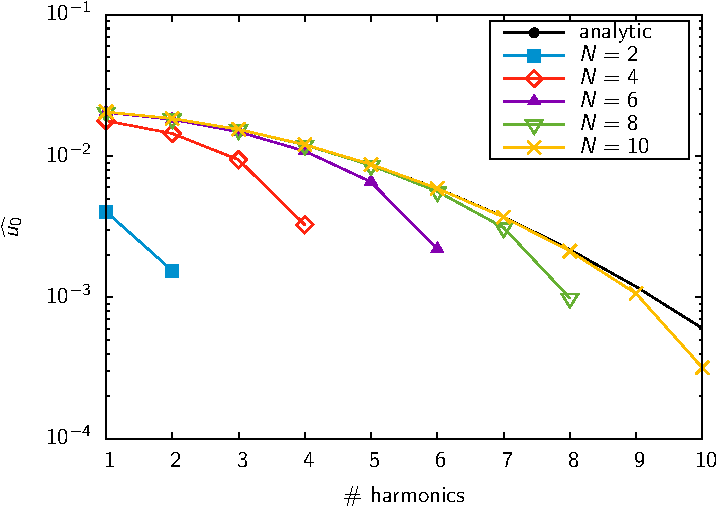
\includegraphics[width=.5\textwidth]{convection_wake_dft.pdf}
  \caption{Linear advection of a Gaussian function representing a turbomachinery wake: 
  discrete Fourier transform.}
  \label{fig:dft_wake}
\end{figure}
The discrete Fourier transform of the results is
depicted against the analytical result in Figure~\ref{fig:dft_wake}.
The $N=2$ and $N=4$ computations badly capture the amplitudes of the
resolved harmonics.
Starting from $N=6$, some of the lower 
frequencies are correctly captured, whereas high frequencies are
always under-estimated.
The capture of the amplitudes 
improves when further harmonics are added to the computation.

For a better understanding of the HB convergence behavior, 
we consider the spectral content of the Gaussian wake model. 
Precisely, the Fourier transform $\widehat{g}$ of a Gaussian function $g$
defined as
\begin{equation}
    g(x) = A e^{-\alpha x^2},
    \label{eq:simple_gaussian_function}
\end{equation}
where $A$ and $\alpha$ are constants, is
\begin{equation}
    \widehat{g}(f) = A^\prime e^{-\alpha^\prime f^2},
    \label{eq:fourier_transform_gaussian}
\end{equation}
where
\begin{equation}
  \begin{cases}
    A^\prime=A \sqrt{\frac{\pi}{\alpha}},\\
    \alpha^\prime = \frac{\pi^2}{\alpha}.
  \end{cases}
\end{equation}
For the similarity law of Lakshminarayana and Davino, 
$\alpha$ and $\alpha^\prime$ can be identified as
\begin{equation}
    \alpha =  0.693 \left( \frac{2}{L} \right)^2, \quad
    \alpha^\prime =  \frac{1}{0.693} \left( \frac{\pi L}{2} \right)^2.
    \label{eq:gaussian_params_laksh}
\end{equation}
The exponential factor of the wake law~$\alpha$ is inversely
proportional to its Fourier counter-part~$\alpha'$, meaning that their
width will vary in opposite way: the thinner the wake, the wider its
spectrum and \emph{vice-versa}.

The convergence rate is inherently linked to
the spectrum of the considered unsteady signal.
As for the present case we know the analytical wake spectrum,
we define the theoretical truncation error as the ratio of
the energy contained in the unresolved part 
of the spectrum to the overall energy content of the full spectrum
\begin{equation}
    \varepsilon_{th}(f) = \sqrt{\frac{
        \int_f^\infty | \widehat{g}(\zeta)|^2 \diff \zeta
      }{
        \int_0^\infty | \widehat{g}(\zeta)|^2 \diff \zeta
      }}.
    \label{eq:def_truncation_error}
\end{equation}
Introducing the error function defined as
\begin{equation}
    \erf(x) = \frac{2}{\sqrt{\pi}} \int_0^x e^{-t^2} \diff t,
\end{equation}
and the complementary error function defined as
\begin{equation}
    \erfc(x) = 1 - \erf(x),
\end{equation}
then
\begin{align}
    \int_0^\infty | \widehat{g}(\zeta)|^2 \diff \zeta 
    &= \frac{1}{2} \int_{- \infty}^\infty | \widehat{g}(\zeta)|^2 \diff \zeta \\
    &= \frac{A^{\prime 2}}{2} \sqrt{\frac{\pi}{2 \alpha^\prime}},
\end{align}
and
\begin{equation}
    \int_f^\infty | \widehat{g}(\zeta)|^2 \diff \zeta = 
      \frac{A^{\prime 2}}{2} \sqrt{\frac{\pi}{2 \alpha^\prime}} \erfc (\sqrt{2 \alpha^\prime} f).
\end{equation}
The theoretical truncation error can finally be written as
\begin{equation}
    \varepsilon_{th}(f, L) = \sqrt{\erfc (\sqrt{2 \alpha^\prime(L) } f)}.
    \label{eq:analytical_conv}
\end{equation}
One can notice from Eq.~\eqref{eq:analytical_conv} that the 
truncation error does not depend on the wake deficit $\Delta u$ 
but only on the wake width $L$.

\begin{figure}[htp]
    \centering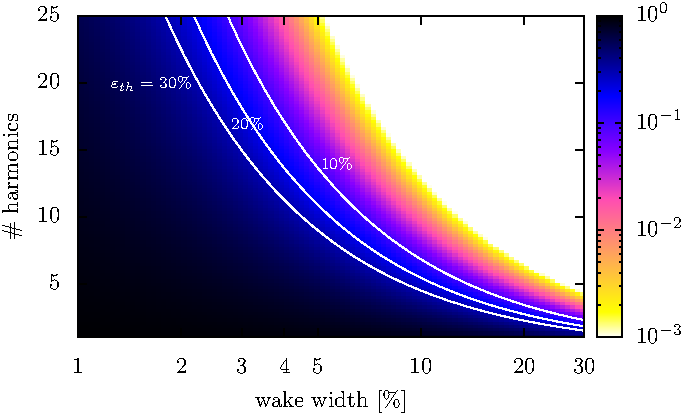
\includegraphics[width=.5\textwidth]{ANALYTICAL_ERROR_PPT.pdf}
  \caption{Theoretical truncation error of the Lakshminarayana and Davino wake law.}
  \label{fig:analytic_error_paper}
\end{figure}
Eq.~\eqref{eq:analytical_conv} is depicted in
Figure~\ref{fig:analytic_error_paper} for varying
numbers of harmonics and wake widths.
It can be seen that the wider the spectrum,
the higher the number of harmonics needed to
reach a certain level of error. 
Moreover, for a thin wake width (\emph{e.g.} 2\% of the pitch)
the number of harmonics required to capture it with a truncation 
error of 10\% is up to 25~harmonics.
In the limit of $L \to 0$, the wake becomes a Dirac function
which represents the worst possible case, as the rectangular
function was.
In the preceding example, the Gaussian function had a width
of 10\% which, according to Eq.~\eqref{eq:analytical_conv},
is captured by using $N=7$ harmonics for a target of 10\% error.

This section provided analytical results of the
convergence of Fourier-based time methods 
in the case of wake passing. To confirm these results,
a turbomachinery like model problem
is set up and solved using the Euler equations in
the following section.





% \chconclu{We have seen that the convergence rate 
% of Fourier-based time methods and hence the harmonic balance approach, 
% in terms of harmonics required to describe the solution 
% with a given level of accuracy, depends on the spectral content of the 
% solution itself: Fourier-based time methods are particularly efficient 
% for flow problems characterized by a narrow Fourier 
% spectrum. We show that main source of unsteadiness in 
% turbomachinery flows is due to the relative motion of wakes 
% generated by a given blade row with respect to the downstream row. 
% Statistically speaking, the passing wakes are seen by the downstream 
% row as an azimuthally advected periodic Gaussian pulse, 
% characterized by its relative thickness compared to the pitch 
% in between two subsequent blades and by the velocity deficit 
% associated to it. We show that the narrower the wake, the larger 
% its Fourier spectrum, and the slower the convergence of Fourier-based time methods.
% In order to achieve \emph{a priori} estimates of the number of 
% harmonics required to accurately solve a given turbomachinery 
% problem, we introduce two error measures based on the relative 
% thickness of the passing wakes. It is shown that, for practical 
% purposes, these can be preliminarily estimated by running a 
% companion steady simulation of the turbomachinery stage. The 
% steady simulation is post-processed to extract information about 
% the spanwise distribution of wake thickness, and an error criterion 
% is used to estimate the number of harmonics required to resolve 99\% 
% of the energy content associated to the velocity signal. The 
% preliminary step has a negligible cost compared to the overall 
% simulation, since the steady computation is used to initialize 
% the unsteady run, and extraction of wake characteristics takes 
% less than a minute on a single processor. 
% The proposed methodology represents an efficient and reliable 
% operational tool to guide the choice of the number of harmonics 
% for a given turbomachinery problem, and to evaluate beforehand the 
% interest of applying or not a Fourier-based time integration scheme 
% instead of a classical time-marching scheme.}
